\subsection{Appearance Editor}
\label{sec:sf-appearance}
\writer{Monica}

The Appearance Editor is a component that will allow the user to add visual information such as shapes and textures to the Petri net objects to be simulated. The connection between the appearance files and the Petri net objects will be done via the \textit{appearance labels}. 

\subsubsection{Functional Requirements}

\begin{enumerate}
\item The Appearance Editor \textbf{shall} allow the user to link appearance labels to 3D objects by choosing a predefined file.
\item The Appearance Editor \textbf{shall} allow the user to link appearance labels to textures by choosing a predefined file.
\item The Appearance Editor \textbf{shall} create an Appearance file in a format that can be read by the Configuration Editor.
\item The Appearance Editor \textbf{shall} allow the user to load an Appearance file.
\item The Appearance Editor \textbf{shall} allow the user to save an Appearance file.
\item It \textbf{would be nice} to allow the user to load a Petri net file in order to retrieve all the appearance labels.     
\end{enumerate}

\subsubsection{Use cases}

The features described above are shown in Figure~\ref{fig:use-cases-appearance-editor}.

\begin{figure}[htp]
\begin{center}
  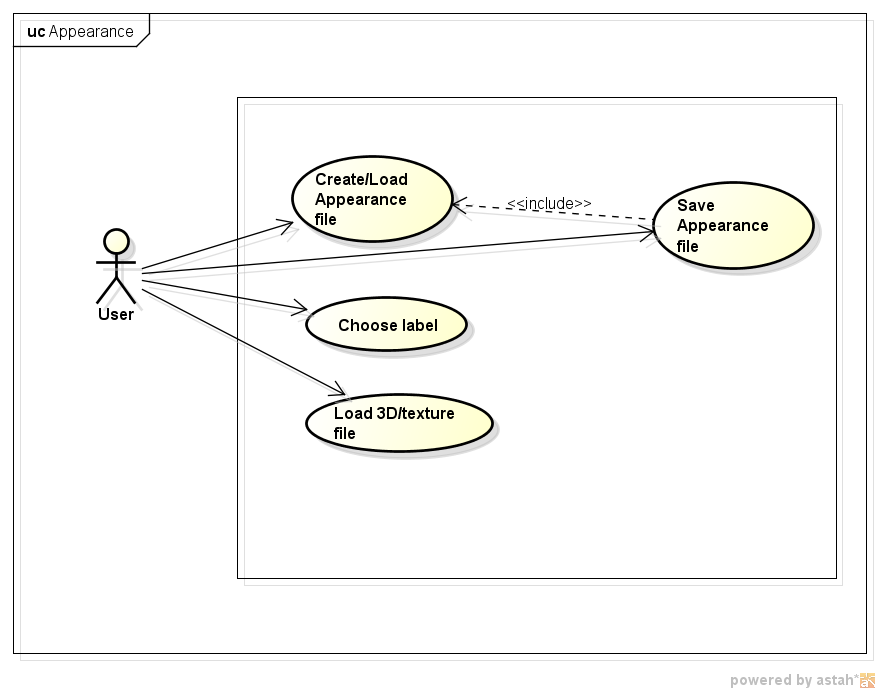
\includegraphics[width=0.5\textwidth]{image/uc-appearance.png}
  \caption{Use cases for the Appearance Editor}
  \label{fig:use-cases-appearance-editor}
\end{center}
\end{figure}

